O tuning do modelo da tarefa anterior foi realizado tendo em conta os parâmetros do número mínimo de registos por nodo, a medida de qualidade
e o método de pruning.

Começando pelo primeiro parâmetro, criei uma variável que itera entre os valores 2 e 10 (de 1 em 1) e associei-a ao respetivo parâmetro no nodo \textit{Decision Tree Learner}

\begin{figure}[H]
    \centering
    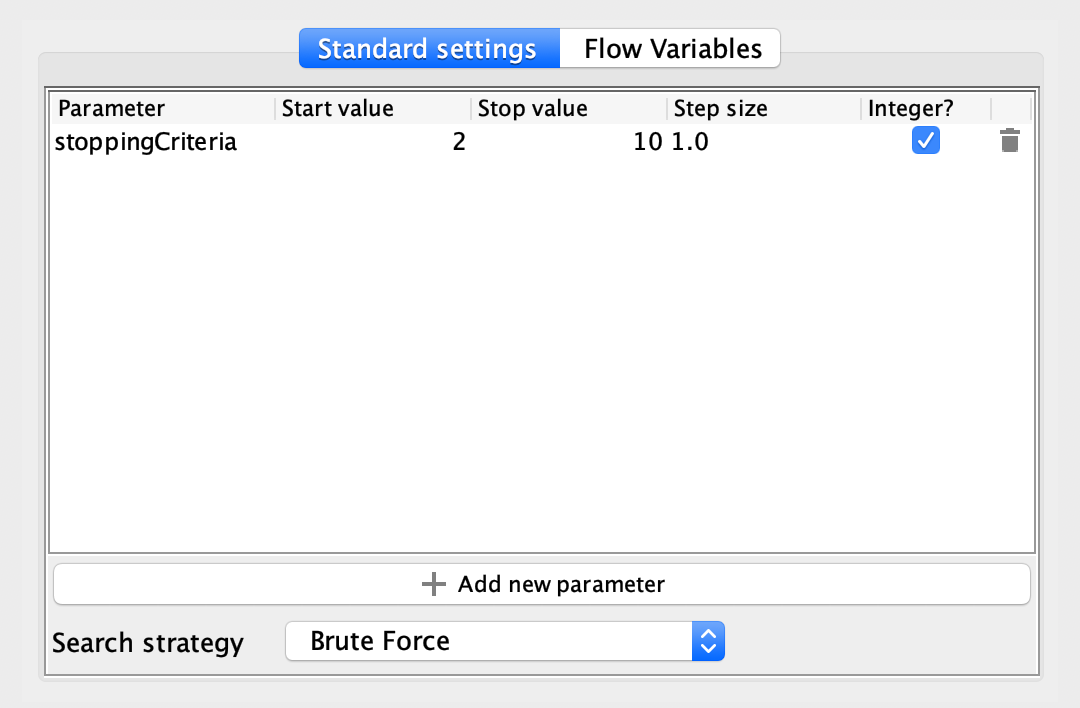
\includegraphics[scale=0.4]{Images/T4_a1.png}
    \caption{Nodo Parameter Optimization Loop Start}
\end{figure}

\begin{figure}[H]
    \centering
    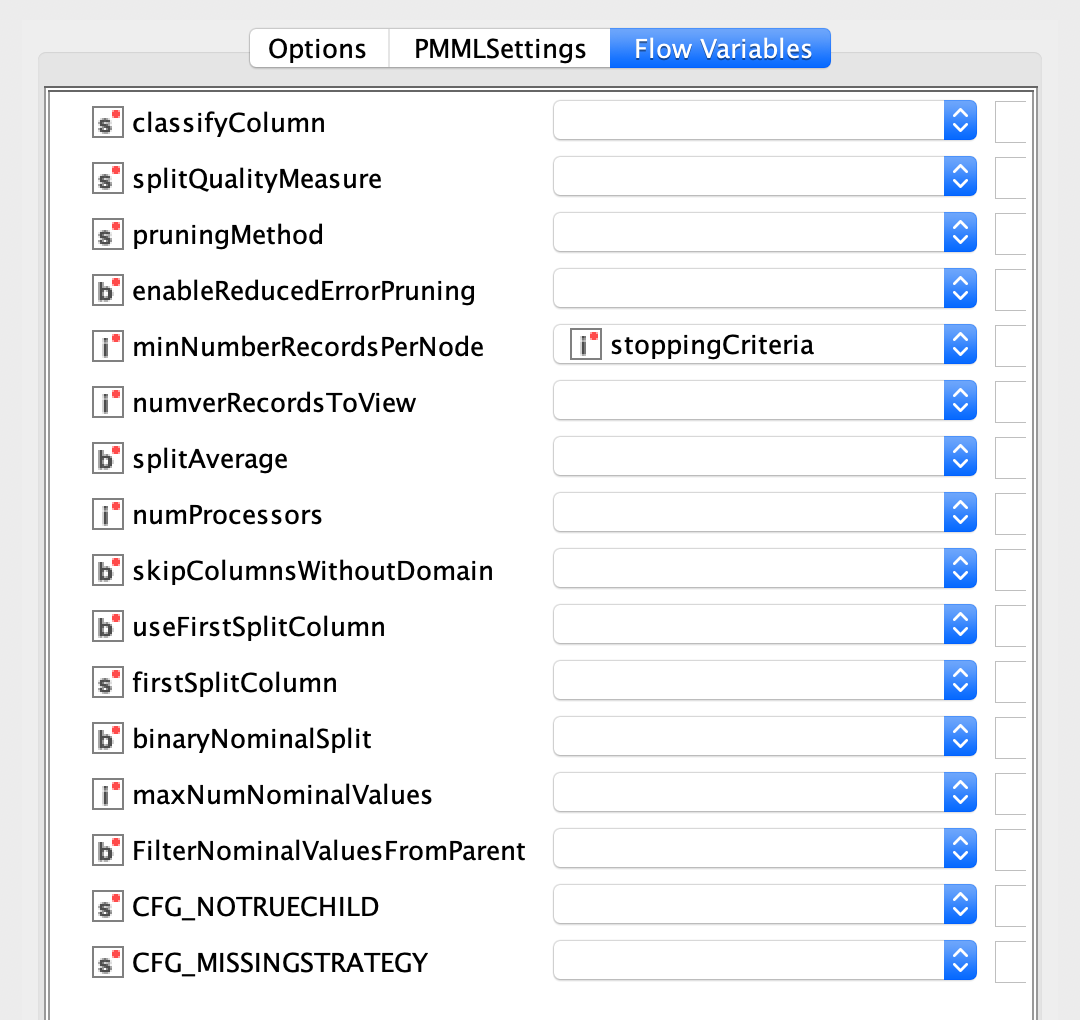
\includegraphics[scale=0.4]{Images/T4_a2.png}
    \caption{Nodo Decision Tree Learner}
\end{figure}

\begin{figure}[H]
    \centering
    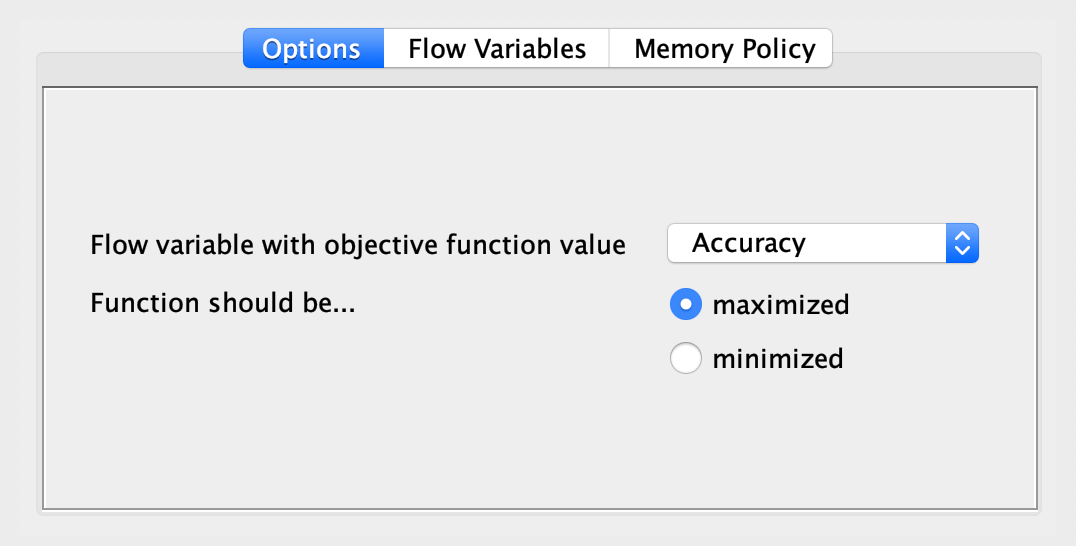
\includegraphics[scale=0.4]{Images/T4_a3.png}
    \caption{Nodo Parameter Optimization Loop End}
\end{figure}

O seguinte \textit{workflow} representa todos os passos realizados.

\begin{figure}[H]
    \centering
    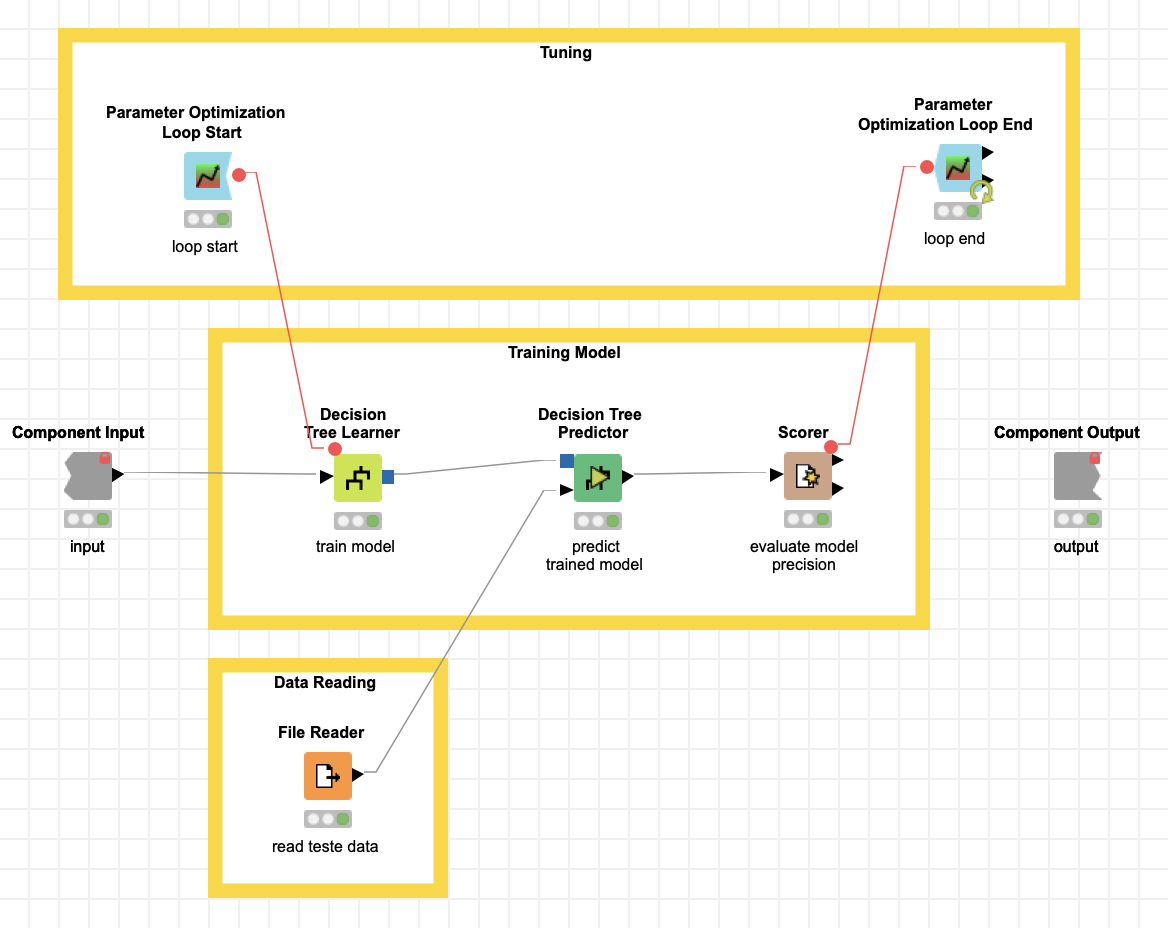
\includegraphics[scale=0.4]{Images/T4_a4.png}
    \caption{Tuning do modelo}
\end{figure}

Para o segundo parâmetro, criei duas colunas cujos valores são as opções para a medida de qualidade e as opções para o método de pruning respetivamente e associei-as aos respetivos parâmetros no nodo \textit{Decision Tree Learner}

\begin{figure}[H]
    \centering
    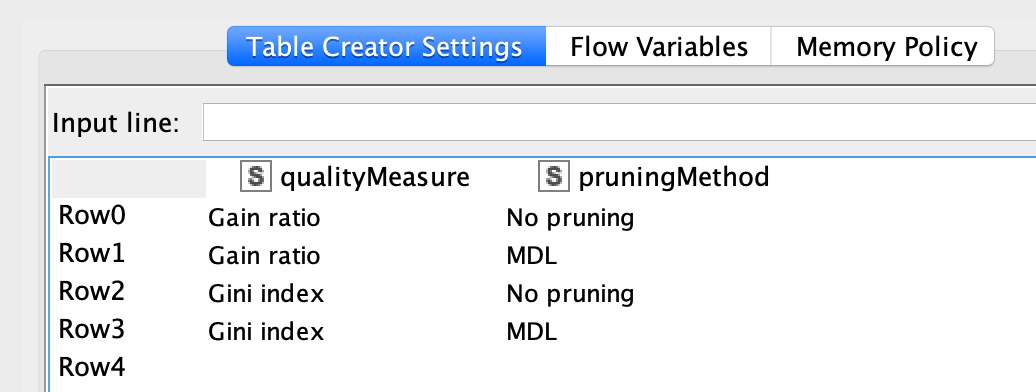
\includegraphics[scale=0.4]{Images/T4_b1.png}
    \caption{Nodo Table Creator}
\end{figure}

\begin{figure}[H]
    \centering
    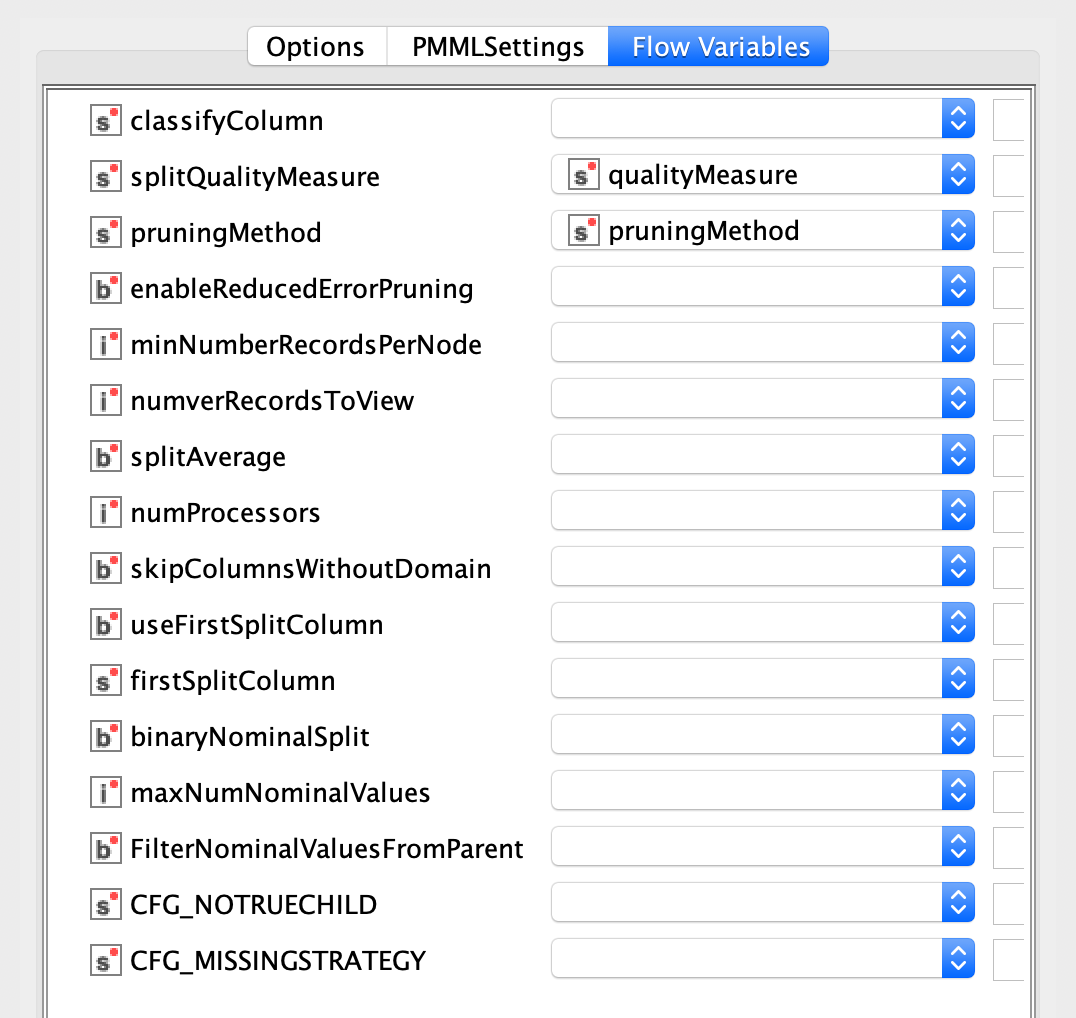
\includegraphics[scale=0.4]{Images/T4_b2.png}
    \caption{Nodo Decision Tree Learner}
\end{figure}

\begin{figure}[H]
    \centering
    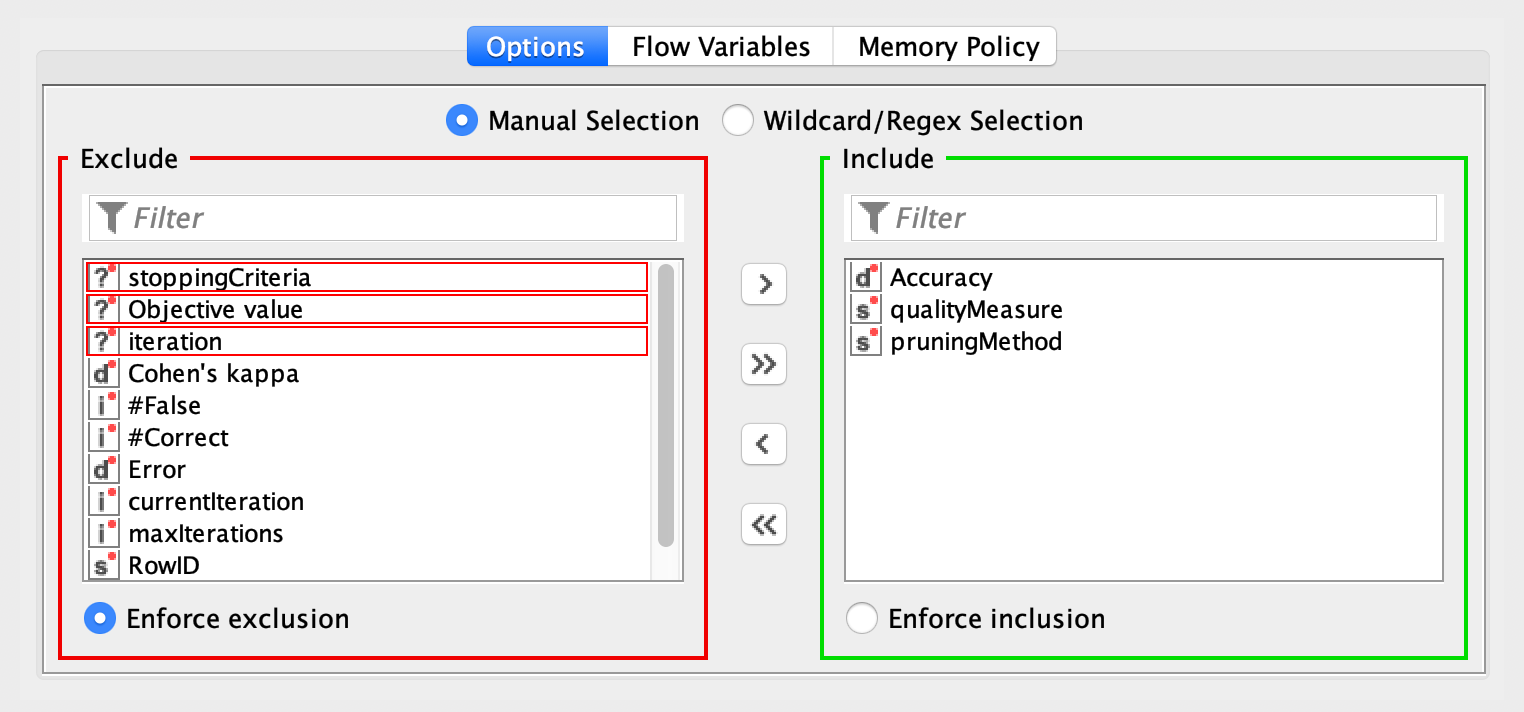
\includegraphics[scale=0.4]{Images/T4_b3.png}
    \caption{Nodo Variable Loop End}
\end{figure}

\clearpage

O seguinte \textit{workflow} representa todos os passos realizados.

\begin{figure}[H]
    \centering
    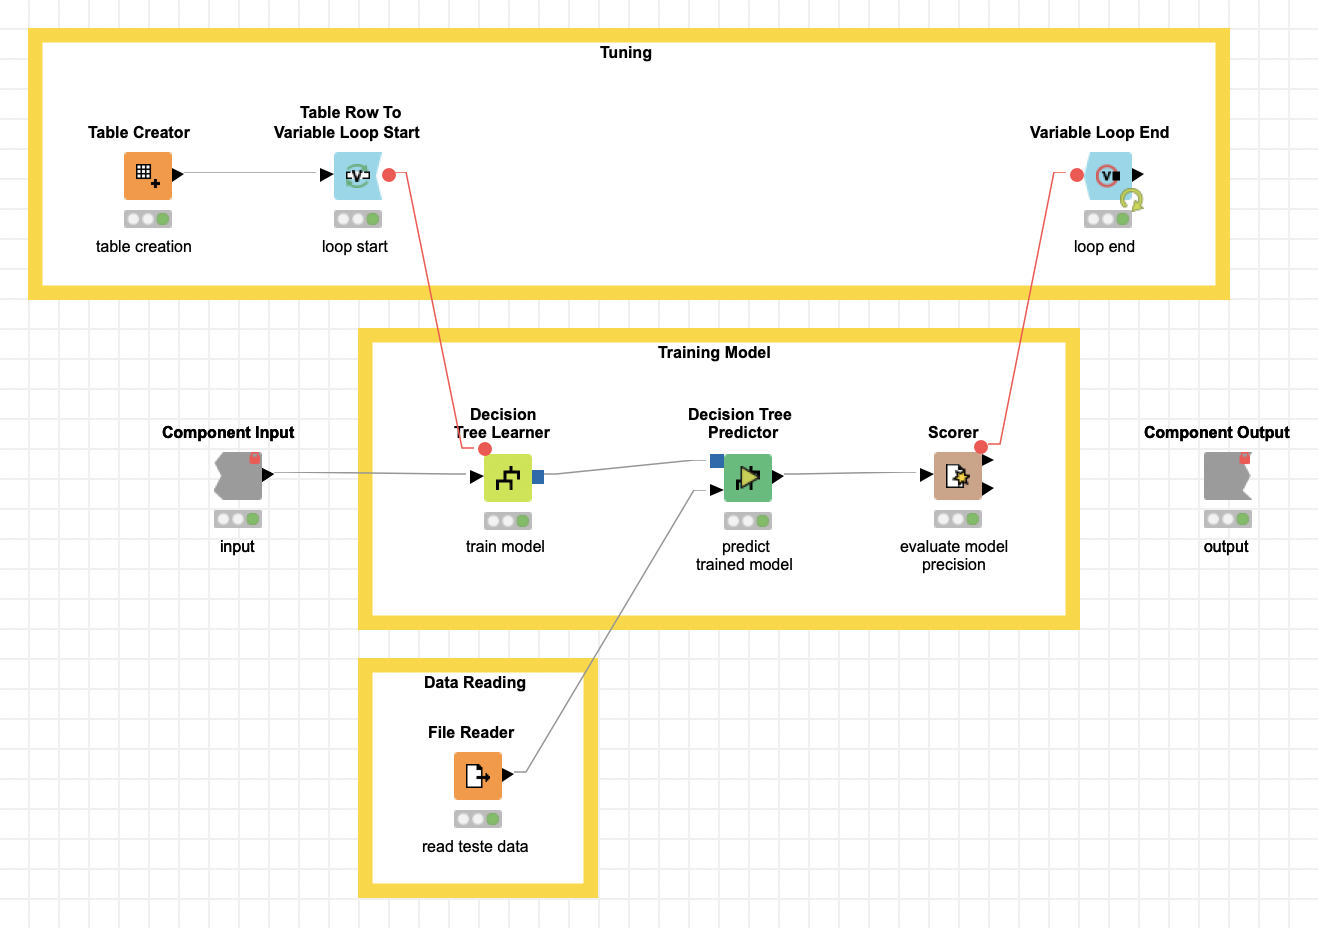
\includegraphics[scale=0.4]{Images/T4_b5.png}
    \caption{Workflow}
\end{figure}

Combinado os tunings anteriores desenvolvi o seguinte \textit{workflow}.

\begin{figure}[H]
    \centering
    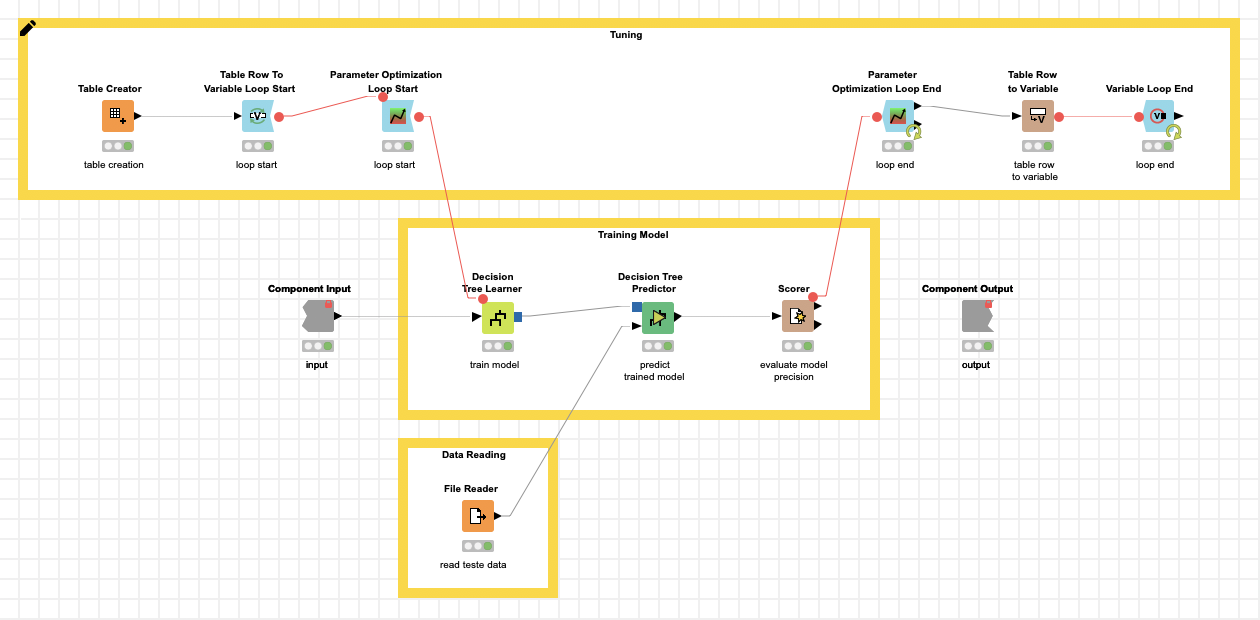
\includegraphics[scale=0.4]{Images/T4_c1.png}
    \caption{Workflow}
\end{figure}

\begin{figure}[H]
    \centering
    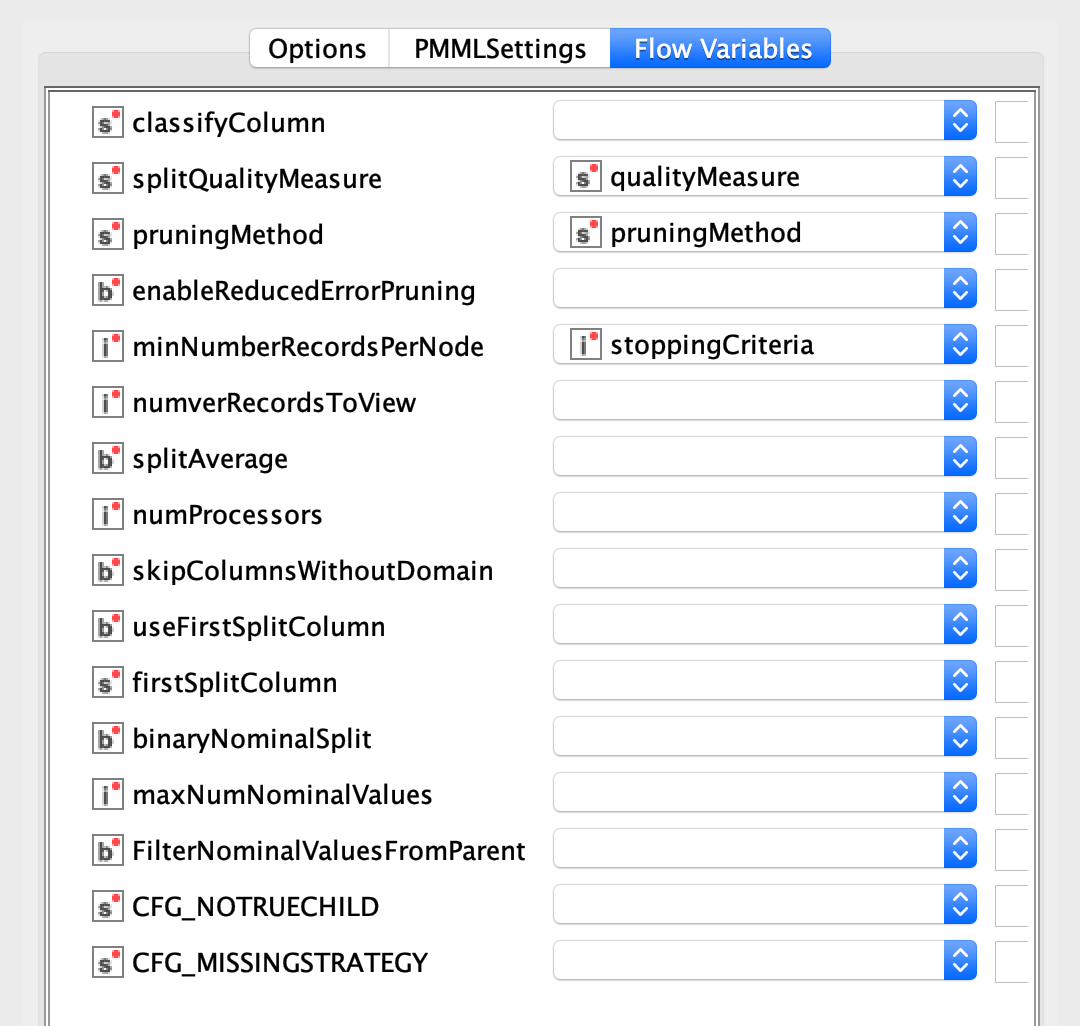
\includegraphics[scale=0.4]{Images/T4_c2.png}
    \caption{Nodo Decision Tree Learner}
\end{figure}

\begin{figure}[H]
    \centering
    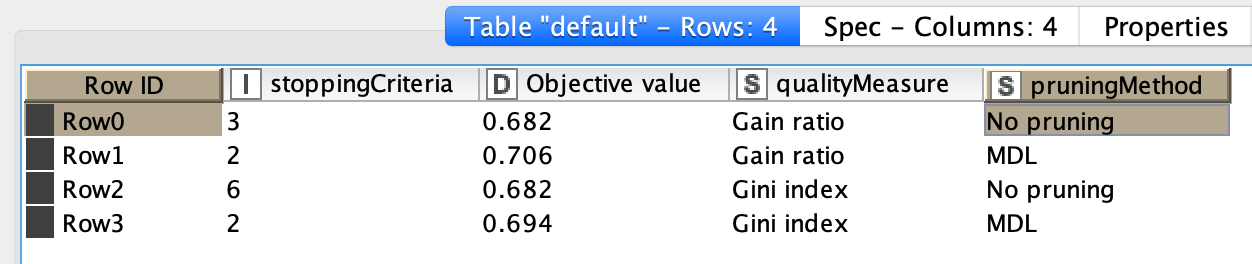
\includegraphics[scale=0.4]{Images/T4_c3.png}
    \caption{Tabela resultante}
\end{figure}

Observando a tabela resultante do pruning do modelo, podemos concluir que a melhor combinação de parâmetros para maximizar a \textit{accuracy} é 2 registos mínimos por nodo, a medida de qualidade \textit{Gain ratio} e método de pruning \textit{MDL}.
Apesar de não haver grandes discrespâncias entre os valores, as diferenças são significativas, especialmente quando o modelo é exposto a um dataset com um maior número de instâncias.